\documentclass[11pt, oneside]{article}   	% use "amsart" instead of "article" for AMSLaTeX format
\usepackage{geometry}                		% See geometry.pdf to learn the layout options. There are lots.
\geometry{letterpaper} 
\usepackage[utf8]{inputenc}                  		% ... or a4paper or a5paper or ...
%\geometry{landscape}                		% Activate for rotated page geometry
%\usepackage[parfill]{parskip}    		% Activate to begin paragraphs with an empty line rather than an indent
\usepackage{graphicx}				% Use pdf, png, jpg, or eps§ with pdflatex; use eps in DVI mode
\usepackage{float} 								% TeX will automatically convert eps --> pdf in pdflatex		
\usepackage{amsmath}

%SetFonts

%SetFonts


\title{Delivery Exercise A: UNIK4150}
\author{Rikesh Chauhan}
%\date{}							% Activate to display a given date or no date

\begin{document}
\maketitle

\section{Propagation basics}
\subsection*{1 a)}
$EIRP$ stands for effective isotropic radiated power. It is the measure of how much power is radiated by an antenna equally in all direction in reference with an isotropic antenna. For a transmitter it is denoted as $P_{TI}$,  known as effective isotropic transmit power and for a receiver it is denoted as $P_{RI}$, known as effective isotropic received power. In case of the transmitter, it is given by
\begin{equation}\label{pti}
EIPR =  P_{TI}=\frac{P_TG_T}{L_T}
\end{equation}
And in case of the receiver, it is given by
\begin{equation}\label{pri}
EIPR = P_{RI} = \frac{P_RG_R}{L_R}
\end{equation}
where:
\begin{flalign*}
P_T /P_R &= \text {transmitted/received power} &\\
G_T/G_R&= \text {gain of transmitter/receiver} &\\
L_T/L_R&= \text {feeder loss of transmitter/receiver} &
\end{flalign*}

\subsection*{1 b)}
Some of the important characteristics of antenna are as follows:
\subsubsection*{Radiation intensity}
Radiation intensity, U, is the amount of power radiated from an antenna per unit solid angle. It is given as
\begin{equation*}
U = r^2S = \frac{P}{4\pi}
\end{equation*}
where:
\begin{flalign*}
r &= \text {distance from antenna} &\\
P &= \text {power radiated by antenna} &\\
S &= \text {power density} &
\end{flalign*}

\subsubsection*{Directivity}
Directivity, $D(\theta, \phi$), of an antenna is the measure of radiation intensity in a particluar direction realtive to the the average radiation intensity in all direction or radiation intensity of isotropic antenna. It is given as 
\begin{equation*}
D(\theta, \phi) = \frac{\text{Radiation intensity in direction $(\theta, \phi)$}}{\text{Mean radiation intensity in all direction}}
\end{equation*}

\subsubsection*{Effeciency}
Efficiency, e,  of an antenna is an important parameter which is the ratio of power radiated from the antenna to power accepted by the antenna. It is given as
\begin{equation*}
e = \frac{\text{Power radiated}}{\text{Power accepted by antenna}} = \frac{R_r}{R_r + R_l}
\end{equation*}
where:
\begin{flalign*}
R_r& = \text{radiation resistance} &\\
R_l& = \text{loss resistance} &
\end{flalign*}

\subsubsection*{Power gain}
Power gain, G, of an antenna is the ratio of its radiation intensity to that of an isotropic antenna radiating the same total power. It is generally given as the product of directivity and efficiency.
\begin{equation*}
G(\theta, \phi) = e D(\theta, \phi)
\end{equation*}

\subsection*{1 c)}
Path loss, L, is the ratio of transmitted to received EIPR, ie ratio of effective isotropic transmit power, $P_{TI}$ in equation \ref{pti} to effective isotropic received power, $P_{RI}$ in equation \ref{pri}.
\begin{equation} \label{pathloss}
\text{Path Loss}, L = \frac{P_{TI}}{P_{RI}} = \frac{P_TG_TG_R}{P_RL_RL_T}
\end{equation}
The Friss transmission formula gives the ratio of received and radiated power in free space as 
\begin{equation}  \label{friss}
\frac{P_R}{P_T} = G_RG_T\left(\frac{\lambda}{4\pi r}\right)^2
\end{equation}
So free space path loss can now be obtained by rearranging equation \ref{friss} to get equation \ref{pathloss} as follows
\begin{equation*}
L_{FS} = \frac{P_TG_TG_R}{P_R} = \left(\frac{4\pi r}{\lambda}\right)^2 = \left(\frac{4\pi rf}{c}\right)^2
\end{equation*}
In decibels units, it is 
\begin{equation} \label{lossdb}
L_{FS(dB)} = 32.4 + 20logR_{km} + 20logf_{MHz}
\end{equation}

To find the free space path loss for a 20 GHz link from the geostatinoary orbit to Kjeller in Norway, we take $R_{km} = 6375 km$ and $f_{MHz} = 20\times 10^3 MHz$ and substitue these in equation \ref{lossdb}. The path loss obtained is 194.51 dB.

\subsection*{1 d)}
It is very important to model noise in the receiver becuase the eventual system performance is determined by the signal to noise ratio, $SNR$ of the receiver. 

A satellite receiver system can be considered to be a cascade of many elements. In the cascaded chain, the noise of first element ie antenna adds directly to the noise of the complete system, while subsequent contributions are divided by the gians of earier elements. That is why the satellite receiver system usually has an amplifier very close to the antenna in order to reduce noise power and increase the SNR of the first element in the cascaded chain.

\section{Wire antenna}
\subsection*{2 a)} 
For a wire antenna of length, $ L=2l$  and current distribution 
\begin{equation} \label{current}
I_z(z') = I_0e^{-jk_0z'}
\end{equation}
the electric far field is obtained by integrating equation 4.27 in textbook with current from equation \ref{current} and limit values of $L = -l $ to $L = l $. The final expression is

\begin{equation} 
E_{\theta} = \frac{jZ_0I_0e^{-jk_0r}}{\pi r} \left[\frac{\sin\left(2k_0l\sin ^{2}\left(\frac{\theta}{2}\right)\right)}{k_0\tan\left(\frac{\theta}{2}\right)}\right] \\
\end{equation}

\subsection*{2 b)}
Number of lobes and its expression :(
 
\subsection*{2 c)} 
I used matlab for calculating radiation intensity, $U$, normalised it by dividing it with the highest value and plotted as follows.
\begin{figure} [H]
  \centering 
  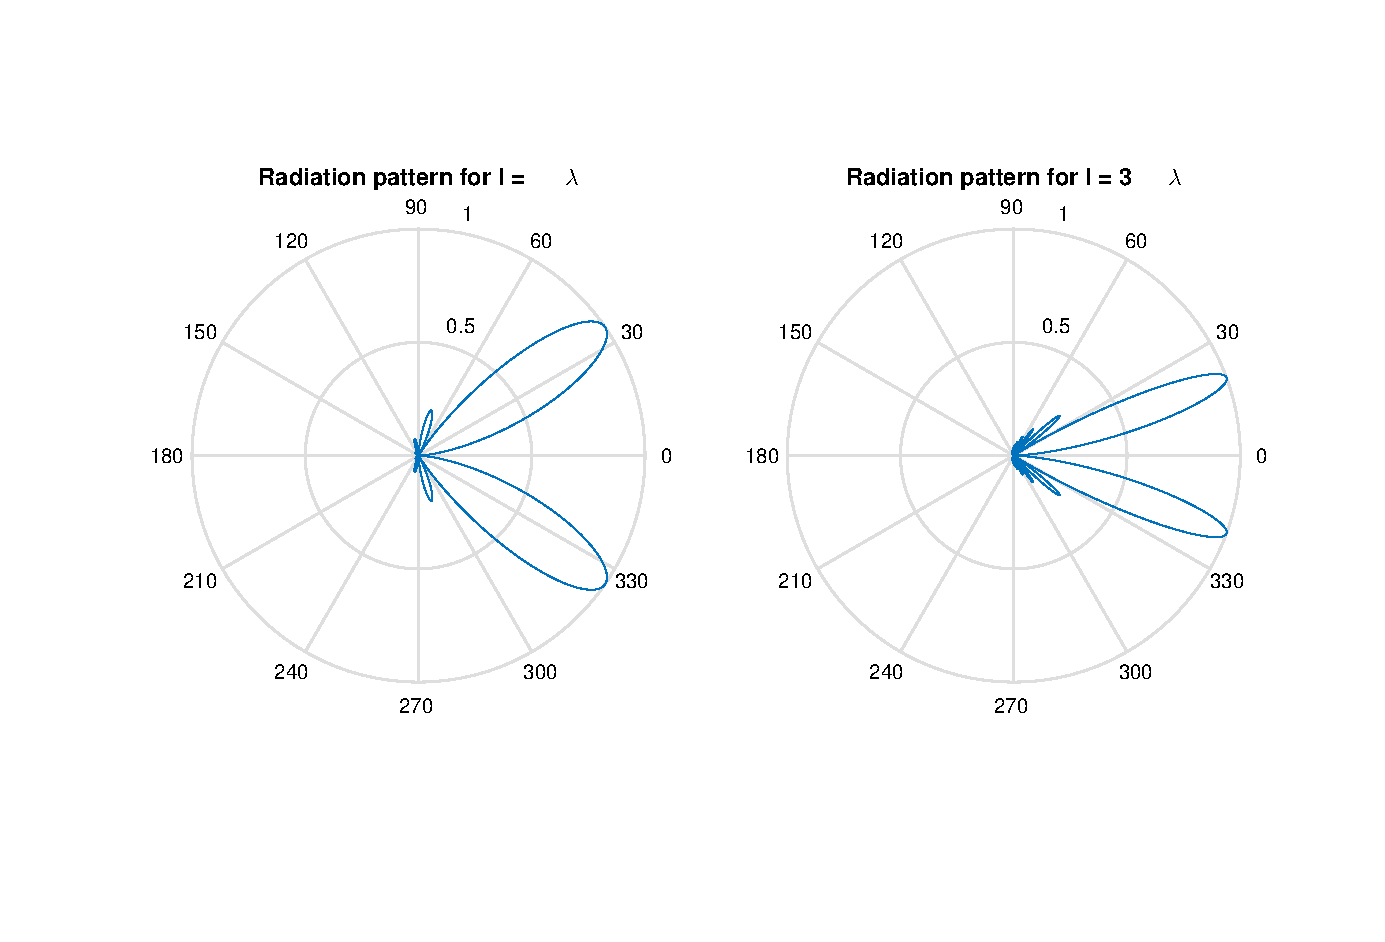
\includegraphics[width=\textwidth]{radiation.eps} 
  \caption{Radiation patterns for current distribution in equation \ref{current}}
  \label{result} 
\end{figure}

\section{Macro cell coverage} 
Given in the question: 95\% successful communication is desired at the fringe of macro cell coverage, and location variability of 6 dB and 10 dB.

\subsection*{3 a)} 
Here we calculate fade margins, $L_s$, also called shadowing loss for $ Q(t) = 10\%$ and $\sigma_L = 6 dB$. \\
From figure 9.5 in the textbook, we find the value of $t$ for  $ Q(t) = 10\%$ which is $t \approx 1.25$\\
Then fade margin is given as 
$$L_s = z = t\sigma_L = 7.5 dB$$
Similarly for  $ Q(t) = 10\%$ and $\sigma_L = 10 dB$, we ger $L_s = 12.5 dB$ \\

\subsection*{3 b)} 
The average availability over the whole cell is given in figure 9.8 and figure 9.9 in the textbook. Since we have already calcuclated the fade margins, we will use figure 9.9 where fade margin is the parameter. The path loss exponent, $n$, is given to be 4.\\

Then for $\sigma_L = 6 dB$, $L_s = 7.5 dB$ is already found.\\
So $\frac{\sigma_L}{n} = 1.5$ Hence from figure 9.9, the average availability is 0.97.\\
Similarly, for $\sigma_L = 10 dB$, the average availability is around 0.95. Since the values in the plot are only given upto $L_s = 10dB$, this value here is approximated from the nature of the plots. 


\subsection*{3 c) }
 If shadowing is neglected in link budget calculations, the maximum acceptable propagation loss is less which in turn increases the maximum system range. This increase in communication range leads to reliability problems, especially at the cell edges.

\end{document}  